% !TeX spellcheck = da_DK
\subsection{Komparator}\label{Komparatorafsnit}
En analog komparator er et kredsløb, der sammenligner en inputspænding eller -strøm med en eller flere referencespændinger eller -strømme. Komparatorens output går fra en mætningsgrænse til en anden, når det negative input af operationsforstærkeren passerer igennem 0 V. Dette betyder, at ved en inputspænding på mere end tærskel niveauet vil outputspændingen opnå negativ mætningsgrad. Omvendt ved en inputspænding, som er lavere end tærskelniveauet, vil output spændingen opnå positiv mætningsgrad \fxnote{skriv hvorfor dette sker rent teknisk}.  Den simpleste komparator er en operationsforstærker. \cite{webster2009} Når accelerometerets signal er blevet behandlet, modtager komparatoren dette. Den vil have nogle indstillede tærskelværdier, og hvis en eller flere af disse opnås, vil komparatoren aktivere de tilknyttede komponenter.\fxnote{kilde - Cecilie} \\
Det kan være fordelagtig at placere modstanden R1 ved inputsignalet, som det kan ses på \figref{komparator}, da dette minimerer overstyringen\fxnote{Et bedre ord end overstyring} af operationsforstærkeren.  Når inputtet, ved en simpel komparator, når tærskelniveauet og der forekommer støj på inputtet, kan outputsignalet svinge kraftigt. Dette kan imidlertid undgås ved at tilføje to modstande, R2 og R3. \cite{webster2009}
\begin{figure}[H]
\centering
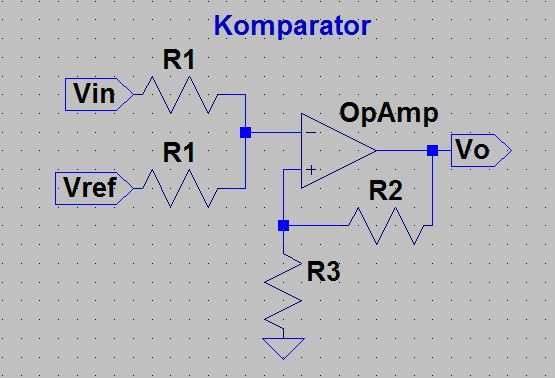
\includegraphics[scale=0.6]{figures/cProblemloesning/Komparator.JPG}
\caption{En simpel komparator, der har fået tilføjet R2 og R3 for at undgå svingninger i outputsignalet. \textit{(Billedet er udarbejdet i LT-spice)}}
\label{komparator}
\end{figure}
